\subsection{Testauswertung}
In diesem Unterkapitel erkläre ich die Implementierung der Input Control und wie sie auf Benutzereingaben korrigiert. Danach zeige ich auf, was mir bei den Performance Tests aufgefallen ist und hebe bestimmte Testergebnisse hervor.

\subsubsection{Verhalten der Input Control}
Bei den Input Control Tests konnte ich aus Zeitgründen nicht alle möglichen Eingabewerte testen. Daher habe ich bei unterschiedlichen input fields variierende Fälle abgedeckt und getestet. Die input fields habe ich selbst bei nummerischen input fields mit einem input type Text HTML-Element implementiert. Nur so konnte ich die Input Control auf die Art und Weise, die ich im Folgenden erklären werde, gestalten. Ich habe absichtlich einige Leerzeichen in die Eingaben eingefügt, um in der Output-Korrektur zu zeigen, dass der white space entfernt wird. Invalid input entsteht, wenn man keine Zahlenwerte in input fields eingibt, die eine Zahl erwarten. In dem Fall bleibt die Eingabe stehen bis der Nutzer sie ändert. Solange invalid input im input field vorhanden ist, ist die zugehörige Operation blockiert. Floats mit Kommas zählen ebenfalls zum invalid input. Man muss stattdessen einen Punkt verwenden, da ich die PDF Web App in Englisch programmiert habe. Eine Ausnahme von blockierten Operationen stellt der Page Counter dar. Hier wird beim Scrollen das invalid input automatisch entfernt und die aktuelle Seite im Viewport erscheint. Die textarea für den benutzerdefinierten Text akzeptiert alle Unicode-Zeichen, falls die Schriftart Unicode unterstützt. Die 14 Standard-Fonts Times Roman (normal, bold, italic), Helvetica (normal, bold, italic), Courier (normal, bold, italic), ZapfDingbats (normal) und Symbol (normal) unterstützen kein Unicode, was ein Resultat der langen Tradition der PDF-Spezifikation ist. Ich habe lediglich alle Times Roman, Helvetica und Courier Schriftschnitte implementiert. Times Roman, Helvetica und Courier unterstützen die WinAnsi Encodierung und ZapfDingbats und Symbol verwenden ihre eigenen spezialisierten Encodings mit 203 und 194 Zeichen \cite{pdf-lib}. Daher sollte man als Benutzer zur Sicherheit immer einen benutzerdefinierten Font verwenden. Ansonsten wird ein Fehler geworfen, der im Screenshot \ref{fig:font-error} gezeigt wird.

\begin{figure}[!htbp]
	\centering
	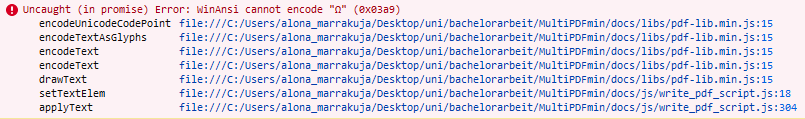
\includegraphics[width=1\textwidth]{"images/font-error.png"}
	\caption{Auftretende Fehlermeldung, wenn der Benutzer bei Verwendung eines PDF Standard-Fonts versucht in die textarea ein Omega-Zeichen einzufügen}
	\label{fig:font-error}
\end{figure}

Das Zoom input field akzeptiert einen Integer mit oder ohne Prozentzeichen. Falls der User kein Prozentzeichen angegeben hat, wird es automatisch hinzugefügt. Das Prozentzeichen dient dazu, dem User einen Hinweis zu geben, dass es sich um eine Zoomfunktionalität handelt. Liegt eine Zahl unter dem minimalen Wertebereich, so wird die Eingabe auf die unterste Schwelle korrigiert. Falls die Zahl über dem maximalen Wertebereich liegt, wird sie auf die oberste Schwelle substituiert. Sowohl bei Integer als auch bei Float input fields kann man bei Werten zwischen -1 und 1 die Null vor dem Dezimalpunkt weglassen oder auch mehrere Nullen schreiben. Im Falle eines Integers wird dann die Eingabe intern als Null interpretiert. Hingegen wird bei einem Float die Null ergänzt bzw. zu einer 0 zusammengefasst. Wird ein Float in einem Integer input field eingegeben, so wird immer abgerundet, d.h. die Zahlen hinter dem Dezimalpunkt werden gelöscht. Die Seitenlisten im Splitter und in den Auswahlfiltern im Editor löschen bei invalid input das Eingabefeld. Man beachte, dass wenn ein geöffnetes PDF mit 11 Seiten im Splitter mit der list of pages zerteilt werden soll und man die Seitenzahl 11 angibt, wird das input field gelöscht, da man ein PDF nicht nach der letzten Seite zerteilen kann. Außerdem werden Dublikate entfernt und die Seitenzahlen werden in aufsteigender Reihenfolge sortiert. Die korrigierte Eingabe substituiert dann die Benutzereingabe, falls die Eingabe valide war. 

\subsubsection{Interpretation der Performance Tests}
Die Testergebnisse der Performance Tests zeigen, dass die Renderdauer maßgeblich von der Dateigröße abhängt. Das größte PDF mit 167,05 MB hat nur 50 Seiten, jedoch gehört es zu den PDFs die am längsten Zeit benötigen im Reader gerendert zu werden. Die Renderdauer von 1,67 Minuten vom PDF mit 850 Seiten ist am höchsten. Es benötigt sogar ungefähr 1 Minute mehr Zeit als das leere PDF mit den 5000 Seiten, was ich im Creator erstellt habe. PDFs mit mehr als 1000 Seiten gehen in den Sekundenbereich.
\par 
Bei den Creator Tests fällt auf, dass das Format sich kaum auf die Ausführungszeit auswirkt. Eine Seite mit dem größten Format, das die PDF Web App unterstützt, liegt von der Speichergröße her im Bytebereich. Man merkt, dass die PDF-LIB für leere PDFs den Speicherplatzbedarf optimiert hat. Auch die Ausführung der Downloadfunktion für die maximale Anzahl an Seiten dauert nur wenige Sekunden. 
\par
In den Testresultaten des Editors fällt auf, dass die Einbettung von 30 Textelementen wesentlich weniger zeitintensiv ist als die Einbettung der anderen Elemente. Geometrieformen und Bilder benötigen fast gleich viel Zeit, während die Zeichnungen am meisten Zeit benötigen. Bilder am Speicher intensivsten und Textelemente verbrauchen wesentlich weniger Speicherplatz als die anderen Elemente.  

